\documentclass[conference,compsoc]{IEEEtran}

% *** CITATION PACKAGES ***
%
\ifCLASSOPTIONcompsoc
  % IEEE Computer Society needs nocompress option
  % requires cite.sty v4.0 or later (November 2003)
  \usepackage[nocompress]{cite}
\else
  % normal IEEE
  \usepackage{cite}
\fi

% *** PDF, URL AND HYPERLINK PACKAGES ***
%
\usepackage{url}
% url.sty was written by Donald Arseneau. It provides better support for
% handling and breaking URLs. url.sty is already installed on most LaTeX
% systems. The latest version and documentation can be obtained at:
% http://www.ctan.org/pkg/url
% Basically, \url{my_url_here}.

\usepackage{adjustbox}
\usepackage{graphicx}
\usepackage{caption}
\usepackage{subcaption}
\usepackage{xcolor}
\usepackage{colortbl}
\usepackage{multirow}
%\usepackage[hyphens]{url}
\usepackage[hidelinks]{hyperref}
\usepackage[nolist]{acronym}
\usepackage{amssymb}
\usepackage{blindtext}
\usepackage{enumitem}
\usepackage{makecell}
\usepackage{listing}
\usepackage{tabularx}
\usepackage{enumitem} % Add labels for RQs defined in enumerated list
\usepackage{amsmath}
\usepackage{balance}

\definecolor{verylightgray}{RGB}{240,240,240}
\definecolor{fuchsia}{rgb}{1.0, 0.0, 1.0}

%% Tikz
\usepackage{tikz}
\usetikzlibrary{positioning, fit} % positioning enables relative positions in tikz, fit enable to create groups of nodes
\usepackage{tikzscale}
\usepackage{pgfplots}
\DeclareUnicodeCharacter{2212}{−}
\usepgfplotslibrary{groupplots,dateplot}
\usetikzlibrary{patterns,shapes.arrows}
\pgfplotsset{compat=newest}

%% Listings
\RequirePackage{listings}
\lstdefinelanguage{Golang}%
    {morekeywords=[1]{package,import,func,type,struct,return,defer,panic,%
    recover,select,var,const,iota,},%
    morekeywords=[2]{string,uint,uint8,uint16,uint32,uint64,int,int8,int16,%
    int32,int64,bool,float32,float64,complex64,complex128,byte,rune,uintptr,%
    error,interface},%
    morekeywords=[3]{map,slice,make,new,nil,len,cap,copy,close,true,false,%
    delete,append,real,imag,complex,chan,},%
    morekeywords=[4]{for,break,continue,range,go,goto,switch,case,fallthrough,if,%
    else,default,},%
    morekeywords=[5]{Println,Printf,Error,Print,},%
    sensitive=true,%
    morecomment=[l]{//},%
    morecomment=[s]{/*}{*/},%
    morestring=[b]',%
    morestring=[b]",%
    morestring=[s]{`}{`},%
}
\lstset{
    frame=none,
    rulecolor=\color{red},
    basicstyle=\footnotesize,
    keywordstyle=\color{blue},
    numbers=left,
    numbersep=5pt,
    showstringspaces=false,
    stringstyle=\color{darkgreen},
    tabsize=4,
    language=Golang,
    xleftmargin=17pt,
    framexleftmargin=27pt,
    framexrightmargin=5pt,
    framexbottommargin=4pt,
    breaklines=true,
    postbreak=\mbox{\textcolor{red}{$\hookrightarrow$}\space},
}

% correct bad hyphenation here
\hyphenation{op-tical net-works semi-conduc-tor}

\newcommand{\todo}[1]{{\color{red}\textbf{Todo: #1}}}
\newcommand{\new}[1]{{\color{blue}#1}}
%\newcommand{\footurl}[1]{{\footnote{\url{#1}}}}
\newcommand{\footurl}[1]{{\footnote{#1}}}

\newcommand{\jl}[1]{{\color{fuchsia}\textbf{Johannes:} #1}}
\newcommand{\lb}[1]{{\color{red}\textbf{Lars:} #1}}
\newcommand{\aw}[1]{{\color{green!60!black}\textbf{Anna:} #1}}

\newcommand{\checkNum}[1]{{\color{red}#1}}


\begin{document}
%
% paper title
% Titles are generally capitalized except for words such as a, an, and, as,
% at, but, by, for, in, nor, of, on, or, the, to and up, which are usually
% not capitalized unless they are the first or last word of the title.
% Linebreaks \\ can be used within to get better formatting as desired.
% Do not put math or special symbols in the title.
\title{A Study of Prevalence, Purpose, and Dangers\\ of Unsafe Go Code in the Wild}


% conference papers do not typically use \thanks and this command
% is locked out in conference mode. If really needed, such as for
% the acknowledgment of grants, issue a \IEEEoverridecommandlockouts
% after \documentclass

% for over three affiliations, or if they all won't fit within the width
% of the page (and note that there is less available width in this regard for
% compsoc conferences compared to traditional conferences), use this
% alternative format:
% 
\author{
\IEEEauthorblockN{
A A\IEEEauthorrefmark{2},
B B\IEEEauthorrefmark{1},
C C\IEEEauthorrefmark{1}, 
Mira Mezini\IEEEauthorrefmark{1}
}
\IEEEauthorblockA{
Technische Universität Darmstadt, D-64289 Darmstadt, Germany\\
}
\IEEEauthorblockA{\IEEEauthorrefmark{1}
E-mail: \{A, B , C, mezini\}@cs.tu-darmstadt.de \\
}
\IEEEauthorblockA{\IEEEauthorrefmark{2}
E-mail: A@cs.tu-darmstadt.de \\
}
}

\newcommand{\toolUsage}{\textit{go-geiger}}
\newcommand{\toolSA}{\textit{go-safer}}
\newcommand{\unsafe}{\textit{unsafe}}

\newcommand{\projsAnalyzed}{\checkNum{343}}
\newcommand{\initalProjs}{\checkNum{500}}
\newcommand{\withoutModules}{\checkNum{150}}
\newcommand{\notCompiled}{\checkNum{7}}

\newcommand{\numberPRs}{\checkNum{14}}
\newcommand{\numberPRsMerged}{\checkNum{10}}
\newcommand{\numberBugsFixed}{\checkNum{60}}

\newcommand{\percentageProjectsWithUnsafe}{\checkNum{38 \%}}
\newcommand{\percentageDependenciesWithUnsafe}{\checkNum{87 \%}}
\newcommand{\percentageProjectsAndDependenciesUnsafe}{\checkNum{91 \%}}

\newcommand{\averageUnsafeImportDepth}{\checkNum{3.08}}
\newcommand{\stdUnsafeImportDepth}{\checkNum{1.62}}

% use for special paper notices
%\IEEEspecialpapernotice{(Invited Paper)}

% make the title area
\maketitle

% As a general rule, do not put math, special symbols or citations
% in the abstract
\begin{abstract}
The Go programming language aims to provide memory and thread safety through compile-time measures such as a strict type system that prevents invalid memory accesses. 
However, it also offers a way of circumventing this safety net through the use of the \unsafe{} package.
While there are legitimate use cases for \unsafe{}, developers must exercise caution to avoid introducing vulnerabilities like buffer overflows or memory corruption in general.
%Common uses for \unsafe{} are efficiency reasons and to create functionality of generics, which are not available in current versions of Go.
%Usages of \unsafe{} may be present not only in a project's source code, but can also be introduced through dependencies.
In this work, we present \toolUsage{}, a novel tool for Go developers to quantify \unsafe{} usages in a projects source code and all of its dependencies.
%Using \toolUsage{}, we conducted a large-scale study on the usage of \unsafe{} in the \projsAnalyzed{} most popular open-source Go projects on GitHub, including a manual analysis of \numberCodeSnippets{} code samples on how \unsafe{} is used.
Using \toolUsage{}, we conducted a study on the usage of \unsafe{} in the top 500 most popular open-source Go projects on GitHub, including a manual analysis of \numberCodeSnippets{} code samples on how \unsafe{} is used.
From the projects using Go's module system  \percentagePackagesWithUnsafe{} of the dependencies contain \unsafe{} usages. 
Of these modularized projects \percentageProjectsWithUnsafe{} contain at least one usage that is not part of the standard library, and \percentageProjectsAndDependenciesUnsafe{} of projects contain at least one \unsafe{} in the project itself or one of its transitive dependencies.
Based on the usage patterns found, we present possible exploit vectors in different scenarios. 
Finally, we present \toolSA{}, a novel static analysis tool to identify dangerous and common usage patterns that were previously undetected with existing tools.

\end{abstract}

% no keywords

% For peer review papers, you can put extra information on the cover
% page as needed:
% \ifCLASSOPTIONpeerreview
% \begin{center} \bfseries EDICS Category: 3-BBND \end{center}
% \fi
%
% For peerreview papers, this IEEEtran command inserts a page break and
% creates the second title. It will be ignored for other modes.
\IEEEpeerreviewmaketitle


\section{Introduction}
\label{sec:intro}

Programming languages with direct memory access through pointers, such as C/C++, suffer from the dangers of memory corruption, including buffer overflows \cite{alnaeli2017, larochelle2001} or \textit{use-after-free} of pointers.
Microsoft, e.g., reports that memory safety accounts for around 70\% of all their bugs\footnote{\url{https://msrc-blog.microsoft.com/2019/07/16/a-proactive-approach-to-more-secure-code/}}. 
To avoid these dangers, many programming languages, such as Java, Rust, Nim, or Google's Go, use automatic memory management and prevent using low-level memory details like pointers in favor of managed object references.
Thus, these languages are memory safe, eliminating most memory corruption bugs. 
However, there are valid use cases for such low-level features.
%Systems languages may need to enforce a specific memory layout to interact with hardware or network protocols, or developers may want to achieve high performance by reusing values in memory without the need or reallocation. 
%Another reason to interact with unmanaged memory is by calling foreign functions of, e.g., a native C library.
%This degree of control over what should happen at program execution is impossible to achieve with the safety measures in place.
%
%The adoption of memory-safe languages for different kinds of applications has been increasing significantly in the last decade. 
%
%While environments and languages such as Java, Rust, Nim or Google's Go try to eliminate many bug classes through their language design and/or runtime, they also provide, to varying degrees, escape hatches to perform potentially unsafe operations.
%if explicitly requested.
%
%To serve these needs
Safe languages therefore provide, to varying degrees, escape hatches to perform potentially unsafe operations.
Escape hatches may be used for optimization purposes, to directly access hardware, to use the foreign function interface (FFI), to access external libraries, or to circumvent limitations of the programming language. 

However, escape hatches may have severe consequences, e.g., they may introduce vulnerabilities.
This is especially problematic when \unsafe{} code blocks are introduced through third-party libraries, and thus \new{are} not directly obvious to the application developer. 
Indeed, a recent study shows that unsafe code blocks in Rust are often introduced through third-party libraries~\cite{evans2020}. 
%Not knowing about the dangers introduced through external dependencies can have severe consequences, e.g., potential vulnerabilities.
\new{Therefore}, security analysts, developers, and administrators need efficient tools to quickly evaluate potential risks in their code base but also the risks introduced by code from others.

In this paper, we investigate Go and the usage of \unsafe{} code blocks within its most popular software projects. 
We developed two specific tools for developers and security analysts.
The first one, called \toolUsage{} (Section~\ref{sec:appr:toolUsage}) analyzes a project including its dependencies for locating usages of the \unsafe{} API and scoring \unsafe{} usages in Go projects and their dependencies. 
It is intended to give a general overview of \unsafe{} usages in a project. % and in which context.

As \unsafe{} usages are benign when used correctly, safe usages of \unsafe{} exist.
\new{However, we identified several commonly used \unsafe{} patterns, e.g., to cast slices and structs, which can break memory safety mechanisms.
They introduce potential vulnerabilities, e.g., by allowing access to additional memory regions. 
We provide insights into the dangers and possible exploit vectors to these patterns, indicating the severe nature of these bugs leading to information leaks or code execution (Section~\ref{sec:appr:vulnerabilites}).
%Therefore, we developed proof-of-concepts for the identified issues, leading to information leaks or code execution.

While the Go tool chain provides a linter, called \textit{go vet}, covering invalid \unsafe{} pointer conversions, 
the linter fails to flag the potentially insecure usages. 
Thus, to support developers we implemented a second tool \toolSA{} (Section~\ref{sec:appr:toolSA}) covering two types of those.}
%However, we identified two patterns which cause potentially dangerous \unsafe{} usages
%and can break the memory safety mechanisms, e.g., by allowing access to additional memory regions via type casts.
%To identify these patterns, we implemented our second tool \toolSA{} (Section~\ref{sec:appr:toolSA}).
%It helps during application development by providing meaningful hints for these usages of \unsafe{} that were previously uncaught with existing tools.

With the help of \toolUsage{}, we performed a quantitative evaluation of the top \initalProjs{} most-starred Go projects on GitHub to see how often \unsafe{} is used in the wild (Section~\ref{sec:eval:unsafewild}). 
Including their dependencies, we analyzed more than \packagesAnalyzedRounded{} individual packages. % for usage of \unsafe{}.
We found that \percentageProjectsWithUnsafe{} of projects contain \unsafe{} usages in their direct application code, and \percentageProjectsAndDependenciesUnsafe{} of
projects contain \unsafe{} usages either in first-party or imported third-party libraries.

We also created a novel data set with \checkNum{1,400} labeled occurrences of \unsafe{}, providing insights into the motivation for introducing \unsafe{} in the source code in the first place (Section~\ref{sec:eval:labeledData}). 
\new{Finally, we used \toolSA{} to find instances of our identified dangerous usage patterns within the data set.}
So far, in the course of this work we submitted \numberPRs{} pull requests to analyzed projects and libraries, fixing over \numberBugsFixed{} individual potentially dangerous \unsafe{} usages \new{(Section~\ref{sec:discussion})}. % \new{ as presented in Section~\ref{sec:discussion}}.

In this paper, we make the following contributions:
%
\begin{itemize}
\item \toolUsage{}, a first-of-its-kind tool for detecting and scoring \unsafe{} usages in Go projects and their dependencies,
\item a novel static code analysis tool, \toolSA{}, to aid in identifying potentially problematic \unsafe{} usage patterns that were previously uncaught with existing tools,
\item a quantitative evaluation on the usage of \unsafe{} in \projsAnalyzed{} top-starred Go projects on GitHub,
\item a novel data set with \checkNum{1,400} labeled occurrences of \unsafe{}, providing insights into what is being used in real-world Go projects and for what purpose, and
\item evidence on how to exploit \unsafe{} usages in the wild.
\end{itemize}

%The paper is organized as follows:
%Section~\ref{sec:background} gives a short introduction to \unsafe{} usage in Go code.
%We discuss \unsafe{} code patterns including possible exploit vectors in Section~\ref{sec:appr}, and present the design and implementation of our tools \toolUsage{} and \toolSA{}. 
%In Section~\ref{sec:eval}, we present our study on unsafe Go code in the wild.
%Then, Section~\ref{sec:discussion} discusses our approach and the study results, including potential threads to validity.
%Section~\ref{sec:rw} discusses related work and Section~\ref{sec:concl} concludes the paper.
\section{Background}
\label{sec:background}

Programming languages that offer direct memory access through pointers, such as C, have traditionally had the problem of a number of common memory vulnerability patterns.
Common problems include buffer overflows \cite{alnaeli2017, larochelle2001} or using pointers after they have been freed.
To reduce this danger, many programming languages like Java or Python use automatic memory management and largely prevent developers from using low-level memory details like pointers in favor of managed object references.

However, there exist valid use-cases for access to such low-level aspects.
Systems languages may need to enforce a specific memory layout in order to interact with hardware or network protocols, or developers may want to achieve high performance by reusing values in memory without the need or reallocation. This degree of control over what is happening at program execution might be impossible with the safety measures in place.

Therefore, some safe languages like Go also include ways to explicitly circumvent the safety measures. The \texttt{unsafe} package in the Go standard library\footnote{\url{https://golang.org/pkg/unsafe}} is a means of doing this. It is a small package that contains three functions \texttt{Sizeof}, \texttt{Alignof}, and \texttt{Offsetof} that are all evaluated at compile time and provide access into memory alignment details of Go data types that would normally be unnecessary to know.
Furthermore, the package provides a pointer type, \texttt{unsafe.Pointer} that allows developers to avoid the restrictions that are in place for regular pointer types.
In particular, it is possible to 

\begin{itemize}
    \item cast any pointer to unsafe.Pointer,
    \item cast unsafe.Pointer to any pointer,
    \item cast unsafe.Pointer to uintptr, and
    \item cast uintptr to unsafe.Pointer
\end{itemize}

The first two rules allow casts between completely arbitrary types, and the other two allow the use of pointer arithmetic.
The usage of the \texttt{unsafe} package removes the safety net provided by the Go type system and compiler, and brings developers down to the flexibility and danger of the pointers in C.

The following two examples show how the \texttt{unsafe} package can be used in practice.
In Listing~\ref{lst:unsafe-ex-in-place-cast}, \texttt{unsafe.Pointer} is used according to rules 1 and 2 to cast the \texttt{in.Items} slice to a new type without reallocating it for efficiency reasons.
The code is taken from the Kubernetes \texttt{k8s.io/apiserver} module with minor adjustments.

\begin{lstlisting}[language=Golang, label=lst:unsafe-ex-in-place-cast, caption=In-Place Cast using the Unsafe Package]
func autoConvert(in *PolicyList, out *audit.PolicyList) error {
	// [...]
	out.Items = *(*[]audit.Policy)(unsafe.Pointer(&in.Items))
	return nil
}
\end{lstlisting}

Listing~\ref{lst:unsafe-ex-escape-analysis} shows how an \texttt{unsafe.Pointer} value can be converted to \texttt{uintptr}, a non-reference type that is large enough to store memory addresses, and back to hide it from the Go escape analysis.

\begin{lstlisting}[language=Golang, label=lst:unsafe-ex-escape-analysis, caption=Hiding a Value from Escape Analysis]
func NoEscape(p unsafe.Pointer) unsafe.Pointer {
	x := uintptr(p)
	return unsafe.Pointer(x ^ 0)
}
\end{lstlisting}

Go uses escape analysis to decide whether variables can be allocated on the stack, or need to be placed on the heap \cite{wang2020}.
Since \texttt{uintptr} values are not regarded as pointer types, storing the address of a pointer in a variable of such a type and then converting it back causes the escape analysis algorithm to miss the chain of references to the underlying value in memory, therefore Go will assume a value does not escape when it actually does, and may place it on the stack.
When developers use this pattern correctly, it can be used for improved efficiency because deallocation is faster on the stack than on the heap.
However, used incorrectly it can cause security problems as described in the next section.


% \subsection{Go Dependency Management}

%Old way: packages, Go Path

%New way: modules, registries, \textit{go.mod} file.

%Package cache, versions, bad reproducibility, relatively high error rates for dependency resolution.

\section{Approach}
\label{sec:impl}
In this section we present problems we identified when using unsafe plus information on how to exploit these issues in the wild.
Furthermore, we present our two tools, \toolUsage{} and \toolSA{}, that aid in locating, evaluating and fixing potentially dangerous unsafe usages in source code.

\subsection{Usage and Security Problems}
In this section, we discuss potential threat models and exploit vectors against real-world \unsafe{} Go code.

\subsubsection*{Garbage Collector Race}

\begin{itemize}
    \item Very short background on garbage collector
    \item Explain race and potential use-after-free with code pattern
    \item Explain threat model, such as information leak
\end{itemize}


\subsubsection*{Escape Analysis Flaw}

\begin{itemize}
    \item Very short background on escape analysis in context of Go
    \item Example code that incorrectly allocates on the stack instead of heap when using flawed cast pattern
    \item Explain threat model
\end{itemize}

\begin{lstlisting}
func main() {
	stringResult := GetString()
	fmt.Printf("main:%s\n", stringResult) // expected (but failed) stdout is "abcdefgh"
}

func GetString() string {
	b := []byte{97, 98, 99, 100, 101, 102, 103, 104}
	out := BytesToString(b)
	fmt.Printf("GetString:%s\n", out) // expected stdout is "abcdefgh"
	return out
}

func BytesToString(b []byte) string {
	bytesHeader := (*reflect.SliceHeader)(unsafe.Pointer(&b))
	strHeader := reflect.StringHeader{
		Data: bytesHeader.Data,
		Len:  bytesHeader.Len,
	}
	return *(*string)(unsafe.Pointer(&strHeader))
}
\end{lstlisting}


\subsubsection*{Implicit Read-Only}

\begin{itemize}
    \item Very short background on ELF sections and read-only property of strings
    \item Explain potential bugs (crashed) due to unnecessary complexity with in-place string casts and mutability
    \item Trade-off: performance vs. developer complexity / explicit code / potential future crashed that are hard to debug
\end{itemize}

We submitted \numberPRs{} pull requests to fix more than \numberBugsFixed{} bugs. \numberPRsMerged{} had already been accepted by the submission of this paper.


\subsection{\toolUsage{}: Automatic Identification of Unsafe Usage}

\subsubsection*{Package Identification and Unsafe Discovery}

We use the Go tool chain to identify the root module of every project, that is the module that is defined by the top-level \textit{go.mod} file in the project.

Then, we enumerate the transitive dependency packages of the project, and build the import tree. Using this import tree, we can identify the import depth as minimum depth in the tree for each package.

For each package, we then parse the code and run static code analysis on the Abstract Syntax Tree (AST). We identify usages of the following \unsafe{} tokens: \textit{unsafe.Pointer}, \textit{unsafe.Sizeof}, \textit{unsafe.Offsetof}, \textit{unsafe.Alignof}, \textit{reflect.SliceHeader}, \textit{reflect.StringHeader}, \textit{uintptr}.
We count all usages, splitting them up in the data set by their usage context as \textit{assignment}, \textit{function declaration}, \textit{call}, \textit{variable declaration}, or \textit{other}.
We save all findings including a context of some code lines for further inspection into CSV files.

\subsection{\toolSA{}: An Unsafe-focused Linter}

\section{A Study of Go's \unsafe{} Usages in the Wild}
\label{sec:eval}


We designed and performed a study of Go \unsafe{} usage to answer the following research questions:

\begin{enumerate}[leftmargin=*,label={RQ\arabic*}]
    \item How prevalent is \unsafe{} in Go projects? \label{rq:prevalApp}
    \item How deep are \unsafe{} code packages buried in the dependency tree? \label{rq:depsDepth}
    \item Which \unsafe{} keywords are used most? \label{rq:distTypes}
    \item Which \unsafe{} operations are used in practice, and for what purpose? \label{rq:purpose}
\end{enumerate}

%Figure~\ref{fig:study-overview} provides an overview of our study methodology.
%\begin{figure}[ht]
    
\includegraphics[width=\textwidth]{assets/figures/study-methodology.pdf}
    \caption{Overview of our Study Methodology}
    \label{fig:study-methodology}
\end{figure}


In the following, we first describe our evaluation data set and then provide in-depth analyses of \unsafe{} usage in the wild using \toolUsage{}.
% of how prevalent \unsafe{} is in the wild, in which way and why it is used in our test data set.
Our evaluation scripts as well as the results are available online\footnote{\url{https://github.com/stg-tud/unsafe_go_study_results}}.
%for further research.


%% included here for manual positioning one page earlier. Belongs to next section, reposition if needed
\begin{figure*}[!t]
    \vspace{2mm}
    \centering
    %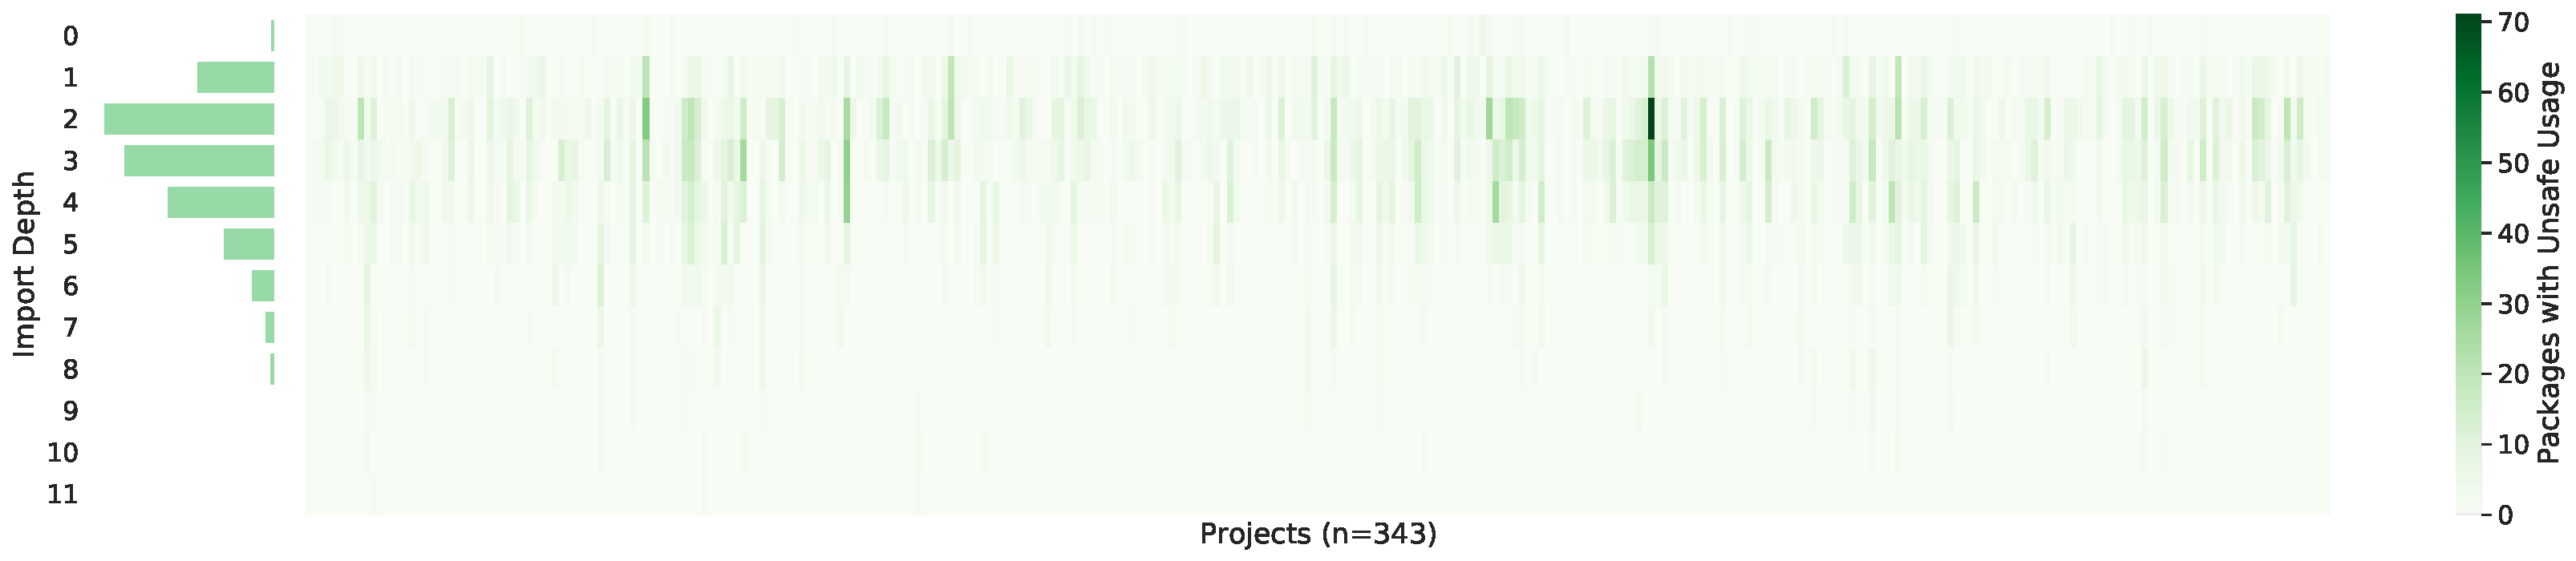
\includegraphics[width=\textwidth]{gfx/figures/unsafe-import-depth.pdf}
    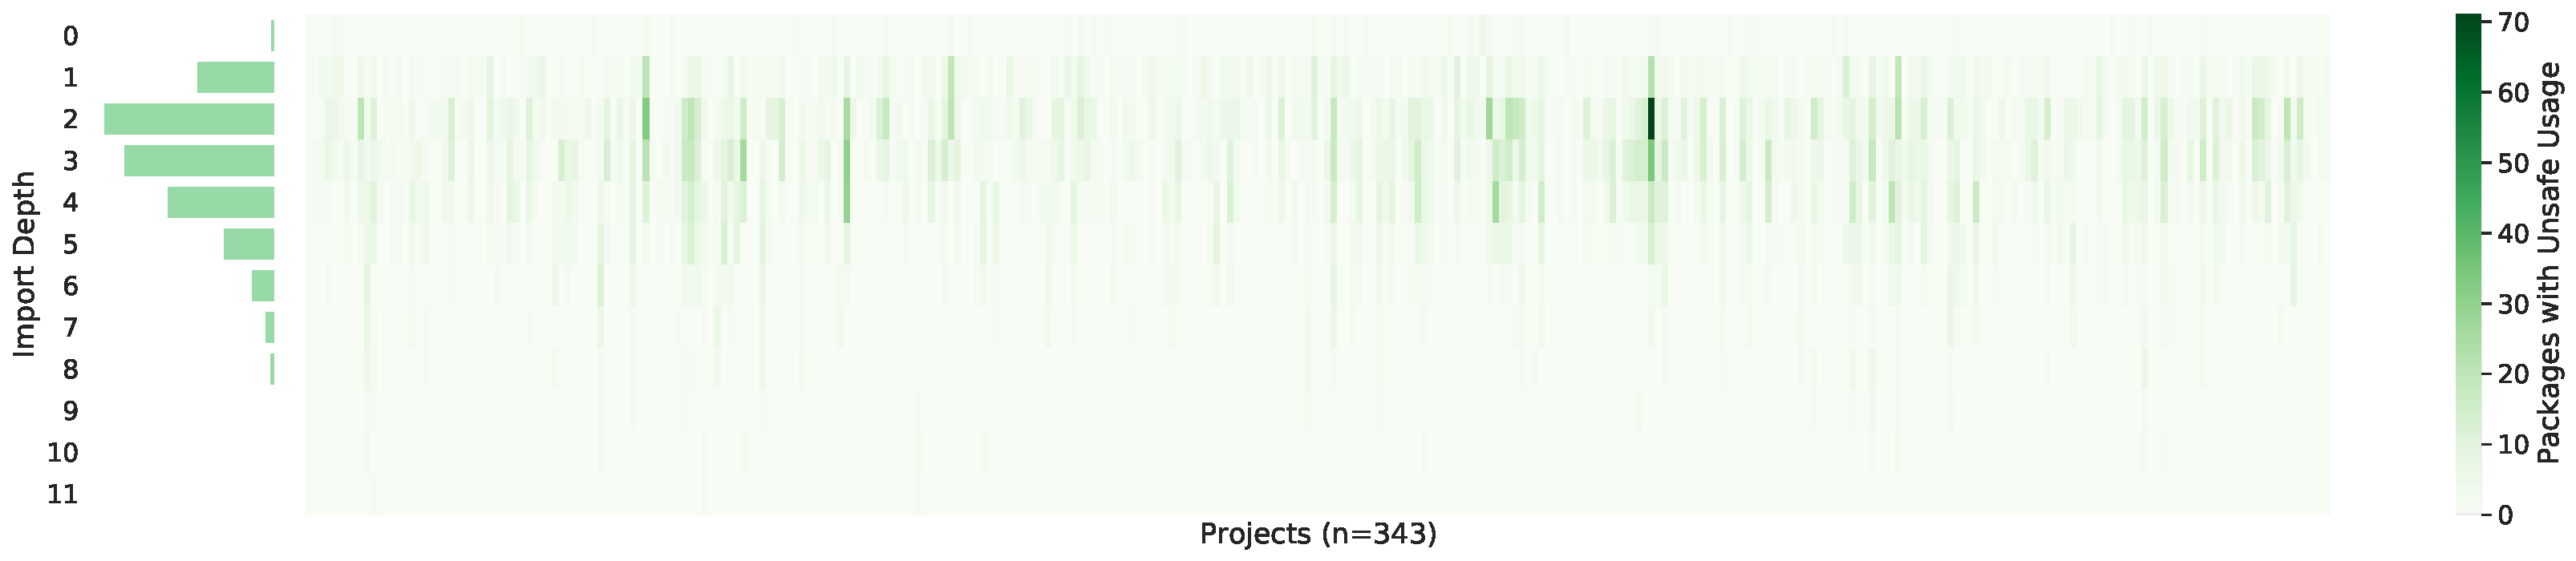
\includegraphics[width=.9\textwidth]{gfx/figures/unsafe-import-depth.pdf}
    \caption{Import Depth of Unsafe Packages. Unsafe packages are around a depth of \averageUnsafeImportDepth{} (sd=\stdUnsafeImportDepth{})}
    \label{fig:unsafe-import-depth}
    %\vspace{-10pt}
\end{figure*}




%% ---------------------------------------------------

\subsection{Data Set}

%For our evaluation, we created a data set of open-source Go code available on GitHub.
As our research is focused on open-source projects, we crawled the \initalProjs{} most-starred Go projects available on GitHub. 
To further understand the influence of dependencies, we then selected the applications supporting \textit{go modules}.
With the introduction of Go \checkNum{1.13}, \textit{go modules}\footnote{\url{https://blog.golang.org/using-go-modules}} are the official way to include dependencies.
Unfortunately, \withoutModules{} of the projects did not yet support Go modules.
Thus, we excluded them from our set.
Furthermore, \notCompiled{} projects that did not compile were also removed.
As a result, we ended up with \projsAnalyzed{} top-rated Go projects. % collected from GitHub.
These have between 72,988 and 3,075 stars, with an average of 7,860. % and median of 5,345. %, thus, this evaluation focuses on very popular projects.
%and save all findings into CSV files.



%% ---------------------------------------------------

\subsection{Unsafe Usages in Projects and Dependencies}
\label{sec:eval:unsafewild}

We used the Go tool chain to identify the root module of each project. 
This is the module defined by the top-level \textit{go.mod} file in the project.
Then we enumerated the dependencies of the project, and build the dependency tree.
For each package, we used \toolUsage{} to generate CSV reports of the found \unsafe{} usages.
Through these analyses we answer the research questions of how many projects use \unsafe{} either in their own code or dependencies (\ref{rq:prevalApp}), and how deep in the dependency tree are the most \unsafe{} code usages (\ref{rq:depsDepth}). 
By selecting only results from the project root modules, we can easily find out how many applications contain a first-hand use of \unsafe{} code.
Our data shows that \checkNum{131} (\checkNum{38.19\%}) projects have at least one \unsafe{} usage within the project code itself.
By looking closer at the imported packages, we see that \checkNum{3,388} of \checkNum{62,025} (\checkNum{5.46\%}) transitively imported packages use \unsafe{}. 
%Through filtering the imported packages, we find that \checkNum{33} of \checkNum{186} (\checkNum{17.74\%}) used standard library packages contain \unsafe{}.
%There are \checkNum{299} (\checkNum{87.17\%}) projects that have at least one direct dependency to a package that has $\geq 1$ unsafe dependency, however for this number we counted only packages belonging to the project's root module as first-party project code. \jl{Might be wrong numbers}
%If a project is split into several modules that all should be logically viewed as first-party project code, they will inflate this number.
There are \checkNum{312} (\checkNum{90.96\%}) projects that have at least one non-standard-library dependency with \unsafe{} usages somewhere in their dependency tree.
Since all projects include the Go runtime, which uses \unsafe{}, counting it as an \unsafe{} dependency would mean that \checkNum{100\%} of projects transitively include \unsafe{}.
We consider this to be less meaningful, as we assume the Go standard library is well audited and safer to use.

%\begin{tcolorbox}[boxsep=1pt, enlarge top by=5pt, title=Answer to \ref{rq:prevalDeps}]
\begin{tcolorbox}[boxsep=1pt, enlarge top by=5pt, title=Answer to \ref{rq:prevalApp}]
About \checkNum{38\%} of projects directly contain \unsafe{} usages.
Furthermore, about \checkNum{91\%} of projects transitively import at least one dependency that contains \unsafe{}.
\end{tcolorbox}

% Using this tree, we can identify the import depth as minimum depth in the tree for each package.
Figure~\ref{fig:unsafe-import-depth} shows the number of packages with at least one \unsafe{} usage by their depth in the dependency tree for every project on its own as a heatmap, alongside the distribution for all projects combined as bars on the left side.
It is evident that most packages with \unsafe{} are imported early in the dependency tree with an average depth of \averageUnsafeImportDepth{}~and a standard deviation of \stdUnsafeImportDepth{}.
This number is very similar to the overall average depth of imported packages (\averageGeneralImportDepth{}). %, regardless of whether they contain usages of \unsafe{}.
While the packages containing \unsafe{} can be manually found and evaluated, this process requires significant resources to handle the increasing number of packages introduced through each dependency. 
For developers only the first level of dependencies, the ones they added themselves, are really obvious.
On this level, \levelOneImportedUnsafePackagesCount{} out of \ImportedUnsafePackagesCount{} imported packages (\levelOneImportedUnsafePackagesShare{}) contain \unsafe{}.

\begin{tcolorbox}[boxsep=1pt, enlarge top by=5pt, title=Answer to \ref{rq:depsDepth}]
Most imported packages containing \unsafe{} usages are found around a depth of \checkNum{3} in the dependency tree.
\end{tcolorbox}



%% ---------------------------------------------------

\subsection{Types and Purpose of Unsafe in Practice}
\label{sec:eval:labeledData}

This section answers \ref{rq:distTypes} and \ref{rq:purpose}.
%This section answers the research questions which \unsafe{} keywords are used most (\ref{rq:distTypes}), as well as which \unsafe{} operations are used in practice for what purpose (\ref{rq:purpose}).
%
Figure~\ref{fig:unsafe-tokens-distribution} shows the distribution of the different \unsafe{} types in our data set.
Packages that are imported in different versions by the projects are counted once per version, as they might contain different \unsafe{} usages and coexist in the wild.
%We found various different usages of \unsafe{} in the analyzed projects, 
In our data set \textit{uintptr} and \textit{unsafe.Pointer} are used about equally often and by far the most common with almost 100,000 findings. 
Next, \textit{unsafe.Sizeof} is still used a bit ($\sim 3,700$), while the other \unsafe{} types are rarely used~($< 1,000$).

\begin{tcolorbox}[boxsep=1pt, enlarge top by=5pt, title=Answer to \ref{rq:distTypes}]
In the wild, \textit{uintptr} and \textit{unsafe.Pointer} are orders of magnitude more common than other \unsafe{} usages.
\end{tcolorbox}

\begin{figure}[!t]
    \centering
    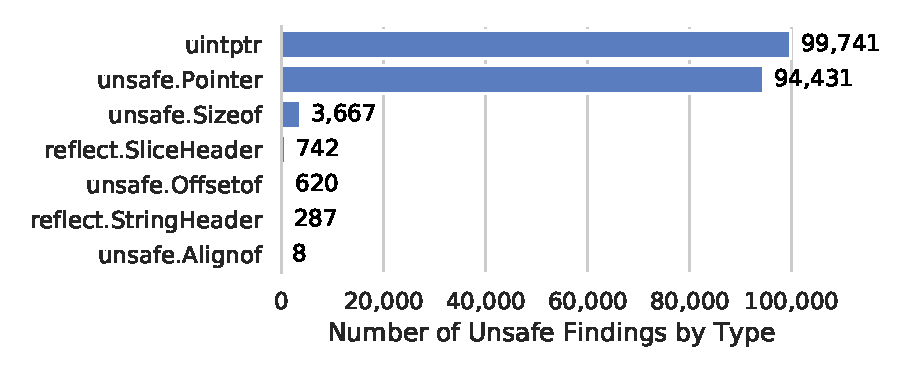
\includegraphics[width=0.43\textwidth]{assets/plots/distribution-unsafe-types.pdf}
    \caption{Distribution of different types of unsafe tokens}
    \label{fig:unsafe-tokens-distribution}
\end{figure}

To learn about the purpose and context in which \unsafe{} is used, we needed to manually analyze code.
Thus, we selected the top \checkNum{10} projects (Table~\ref{tbl:dataset-projects}) with the most \unsafe{} usages in non-standard library packages.
%These projects including the Git revision analyzed plus some additional data are shown in Table~\ref{tbl:dataset-projects}.
From these projects and all their transitive dependencies, we randomly sampled \checkNum{400} code snippets that were found in the \textit{standard library (std)} and \checkNum{1,000} snippets from the remaining packages (\textit{app}).
We define standard library code as all packages that are part of the Go standard library or the \textit{golang.org/x/sys} module, as the \textit{syscall} standard library package is deprecated in favor of this module\footnote{\url{https://golang.org/pkg/syscall}}.
We split the snippets into two groups to analyze if there is a difference between the official standard library and non-standard library code regarding the usage of \unsafe{}.
Then, we identify class labels in two dimensions: what is being done, and for what purpose. 
Finally, we manually analyze all \checkNum{1,400} code snippets and label them accordingly.
The results of this process are shown in Table~\ref{tbl:dataset-classes}.

\begin{table}[!t]
\vspace{2mm}

    \centering
    \caption{Projects selected for labeled data set}
    \label{tbl:dataset-projects}
    \begin{adjustbox}{max width=\textwidth}
    \begin{tabular}{llrrl}
        %\hline
        {} & \textbf{Name} &  \textbf{Stars} &  \textbf{Forks} &    \textbf{Revision} \\ \hline
        \rowcolor{verylightgray}
        1  &         kubernetes/kubernetes &  66,512 &  23,806 &  \texttt{fb9e1946b0} \\
        2  &                 elastic/beats &   8,852 &   3,207 &  \texttt{df6f2169c5} \\
        \rowcolor{verylightgray}
        3  &             gorgonia/gorgonia &   3,373 &    301 &  \texttt{5fb5944d4a} \\
        4  &              weaveworks/scope &   4,354 &    554 &  \texttt{bf90d56f0c} \\
        \rowcolor{verylightgray}
        5  &  mattermost/mattermost-server &  18,277 &   4,157 &  \texttt{e83cc7357c} \\
        6  &               rancher/rancher &  14,344 &   1,758 &  \texttt{56a464049e} \\
        \rowcolor{verylightgray}
        7  &                 cilium/cilium &   5,501 &    626 &  \texttt{9b0ae85b5f} \\
        8  &                     rook/rook &   7,208 &   1,472 &  \texttt{ff90fa7098} \\
        \rowcolor{verylightgray}
        9  &             containers/libpod &   4,549 &    539 &  \texttt{e8818ced80} \\
        10 &                       xo/usql &   5,871 &    195 &  \texttt{bdff722f7b} \\ %\hline
    \end{tabular}
    \end{adjustbox}
    %% reduce space after table for vspace tweaking
    \vspace{-10pt}
\end{table}
\begin{table*}[htp!]
    \centering
    \caption[Labeled unsafe.Pointer usages in application code (non standard library) and standard library samples]
        {Labeled unsafe.Pointer usages in application code (non standard library) and standard library samples~\newline \tiny ~\newline \footnotesize
        \underline{eff}: efficiency, \underline{ser}: (de)serialization, \underline{gen}: generics,
        \underline{no GC}: avoid garbage collection, \underline{atomic}: atomic operations,
        \underline{FFI}: foreign function interface, \underline{HE}: hide from escape analysis, \underline{layout}: memory layout control,
        \underline{types}: Go type system,
        \underline{reflect}: type reflection, \underline{unused}: declared but unused \tiny ~\newline}
    \label{tbl:dataset-classes}
    \begin{adjustbox}{max width=\textwidth}
    
    %% do not paste from notebook, local changes done!
\begin{tabular}{r|cc|cc|cc|cc|cc|cc|cc|cc|cc|cc|cc|cc}
                    & \multicolumn{2}{c|}{\textbf{eff}} & \multicolumn{2}{c|}{\textbf{ser}} & \multicolumn{2}{c|}{\textbf{gen}} & \multicolumn{2}{c|}{\textbf{no GC}} & \multicolumn{2}{c|}{\textbf{atomic}} & \multicolumn{2}{c|}{\textbf{FFI}} & \multicolumn{2}{c|}{\textbf{HE}} & \multicolumn{2}{c|}{\textbf{layout}} & \multicolumn{2}{c|}{\textbf{types}} & \multicolumn{2}{c|}{\textbf{reflect}} & \multicolumn{2}{c|}{\textbf{unused}} & \multicolumn{2}{c}{\textbf{total}} \\ %\hline
                    &  \textbf{app} &  \textbf{std} &  \textbf{app} &  \textbf{std} &  \textbf{app} &  \textbf{std} &   \textbf{app} &  \textbf{std} &    \textbf{app} &  \textbf{std} &  \textbf{app} &  \textbf{std} &  \textbf{app} &  \textbf{std} &    \textbf{app} &  \textbf{std} &   \textbf{app} &  \textbf{std} &     \textbf{app} &  \textbf{std} &    \textbf{app} &  \textbf{std} &   \textbf{app} &  \textbf{std} \\ \hline
                    
                    \textbf{cast} & 562 & 16 & 178 & 33 & 18 & & & & & & 24 & 6 && 2 & 3 & 13 & & 45 & 1 & & & & 786 & 115 \\ 
      %  cast-struct &  401 &    4 &   50 &    6 &    6 &      &       &      &        &      &    6 &    2 &      &    2 &        &    4 &       &   31 &         &      &        &      &   463 &   49 \\
%\rowcolor{verylightgray}
      %   cast-basic &   90 &    2 &   29 &    3 &    1 &      &       &      &        &      &    1 &    3 &      &      &      2 &    7 &       &    1 &         &      &        &      &   123 &   16 \\
      %  cast-header &   36 &    1 &    3 &      &    1 &      &       &      &        &      &      &      &      &      &        &      &       &    3 &         &      &        &      &    40 &    4 \\
%\rowcolor{verylightgray}
      %   cast-bytes &   22 &    1 &   81 &   11 &      &      &       &      &        &      &    1 &      &      &      &      1 &      &       &    1 &         &      &        &      &   105 &   13 \\
      % cast-pointer &   13 &    8 &   15 &   13 &   10 &      &       &      &        &      &   16 &    1 &      &      &        &    2 &       &    9 &       1 &      &        &      &    55 &   33 \\
\rowcolor{verylightgray}
      \textbf{memory-access} &    2 &    1 &    9 &      &      &      &       &      &        &      &      &    1 &      &      &      4 &    6 &       &    4 &         &      &        &      &    15 &   12 \\
 \textbf{pointer-arithmetic} &    7 &    2 &    6 &    1 &      &      &       &      &        &    1 &      &    3 &    1 &    2 &      3 &    8 &       &    9 &         &      &        &      &    17 &   26 \\
\rowcolor{verylightgray}
         \textbf{definition} &    4 &    1 &   23 &      &    2 &      &       &      &        &      &    4 &    5 &      &      &        &    9 &       &    8 &       6 &    3 &        &      &    39 &   26 \\
           \textbf{delegate} &    4 &      &   64 &      &    2 &      &       &      &     11 &    5 &   29 &   45 &      &    4 &        &   14 &       &    6 &         &    1 &        &      &   110 &   75 \\
\rowcolor{verylightgray}
            \textbf{syscall} &      &      &      &      &      &      &    17 &  138 &        &      &      &      &      &      &        &      &       &      &         &      &        &      &    17 &  138 \\
             \textbf{unused} &      &      &      &      &      &      &       &      &        &      &      &      &      &      &        &      &       &      &         &      &     16 &    8 &    16 &    8 \\ \hline
%\rowcolor{verylightgray}
                  \textbf{total} &  579 &   20 &  280 &   34 &   22 &    0 &    17 &  138 &     11 &    6 &   57 &   60 &    1 &    8 &     10 &   50 &     0 &   72 &       7 &    4 &     16 &    8 &  1000 &  400 \\
\end{tabular}

    \end{adjustbox}
        \vspace{-10pt}
\end{table*}

In the following, we outline the identified usage type classes describing what is being done in code.
The most prevalent are \textit{cast} operations from arbitrary types to other structs, basic Go types such as integers, slice/string headers, byte slices, or raw \textit{unsafe.Pointer} values. 
%The most prevalent are \textit{cast-struct}, \textit{cast-basic}, \textit{cast-header}, \textit{cast-bytes}, and \textit{cast-pointer}, which are all cast operations from arbitrary types to other arbitrary structs, basic Go types such as integers, slice or string headers, byte slices, or raw \textit{unsafe.Pointer} values.
The \textit{memory-access} class is applied where \textit{unsafe.Pointer} values are dereferenced, used to manipulate corresponding memory or for comparison with another address.
\textit{Pointer-arithmetic} denotes usages of \unsafe{} to do some form of arithmetic manipulation of addresses, such as advancing an array.
\textit{Definition} groups usages where a field or method of type \textit{unsafe.Pointer} is declared for later usage.
\textit{Delegate} are instances where \unsafe{} is only needed in a function to pass it along to another function requiring a parameter of type \textit{unsafe.Pointer}. 
Thus, the need to use \unsafe{} is actually located elsewhere.
\textit{Syscall} are calls using the Go \textit{syscall} package or \textit{golang.org/x/sys} module.
As the name suggests, \textit{unused} is a class of occurrences that are not actually used in the analyzed code, e.g. dead code or unused parameters.

Our identified purpose classes, providing hints on why \unsafe{} is used, are described in the following.
\textit{Efficiency} includes cases where \unsafe{} is used only for the aim to improve time or space efficiency of the code.
The \textit{serialization} class contains (un)marshalling and (de)serialization operations such as in-place casts from complex types to bytes.
\textit{Generics} applies when \unsafe{} is used to build functionality that would otherwise be solved with generics if they were available in Go.
Samples in the \textit{avoid garbage collection} class are used to tell the Go compiler to not free a value while it is used, e.g., by a function written in assembly.
The \textit{atomic operations} class contains usages of the \textit{atomic} API which expects \unsafe{} for some functions.
The \textit{foreign function interface (FFI)} class contains interoperability with C code (CGo), and calling  functions that expect their parameters as \unsafe{} pointers.
\textit{Hide from escape analysis} includes the pattern described earlier (Listing~\ref{lst:unsafe-ex-escape-analysis}) to break the escape analysis chain.
The \textit{memory layout control} class contains code used for low-level memory management.
\textit{Types} snippets are used by the standard library to implement the Go type system.
\textit{Reflect} includes instances of type reflection and re-implementations of some types of the \textit{reflect} package, e.g. using \textit{unsafe.Pointer} instead of \textit{uintptr} for slice headers.
Again, \textit{unused} is a class of unused occurrences.

%Among the \checkNum{1,400} labeled snippets, \checkNum{683} are located in automatically generated code.
%It might be safe to assume that generated code is less dangerous, however, as bugs in the code generator can have very serious effects of scale, we included them in the study nonetheless.

Using \unsafe{} for the sake of efficiency is the most prevalent motivation to use \unsafe{} in the wild covering \checkNum{58\%} in application code, whereas it is only used for this purpose in \checkNum{5\%} of the cases in std. 
From these, \checkNum{97\%} resp. \checkNum{80\%} are achieved by casting different types. 
The second biggest reason to use \unsafe{} in app is to perform some form of (de)serialization, accounting for \checkNum{28\%}.
%Interestingly, we observe efficiency improvements for \checkNum{4\%} and \checkNum{58\%} of the usages for the standard library and the remaining libraries, respectively.
For the standard library, the most relevant motivation is avoiding garbage collection with \checkNum{35\%}, whereas this is only used in \checkNum{2\%} of the usages in the app sample.
Furthermore, in std type \checkNum{18\%}, FFI \checkNum{15\%} and memory layout \checkNum{13\%} related \unsafe{} usages are rather common.
Both subsets share that hiding from escape analysis with \checkNum{0.1\%} (\textit{app}) and \checkNum{2\%} (\textit{std}) and using \unsafe{} for reflection with \checkNum{1\%} (both) are rare.
%Another interesting observation is that there seem to be two main motivations which occur only for the standard- or 3rd party libraries respectively. 
%Only the standard library makes use of \unsafe{} to implement types being \checkNum{5\%} of the analyzed code snippets. 
%All usages (\checkNum{2\%}) to solve the missing generics functionality in Go are within 3rd party libraries. 
Implementation of generics functionality which is currently missing in Go is only done in few samples (\checkNum{2\%}), although some of the finding in the serialization class could alternatively be achieved with generics as well.

%It is obvious that most of the \unsafe{} found in the wild is used to improve efficiency by casting different types in place, or for fast (un)marshalling operations that would otherwise need either reflection or support for generics.
%Furthermore, \unsafe{} is required to call some functions that expect it, such as atomic operations or certain \textit{FFI} functions.
%The standard library makes extensive use of \unsafe{} to implement types and memory management.
%Hiding values from escape analysis on purpose is done rarely.

\begin{tcolorbox}[boxsep=1pt, enlarge top by=5pt, title=Answer to \ref{rq:purpose}]
\checkNum{More than half} of the \unsafe{} usages in projects and 3rd party libraries are to improve efficiency via \unsafe{} casts.
In the Go standard library, \checkNum{every third} use of \unsafe{} is to avoid garbage collection. 
\end{tcolorbox}


\subsection{Vulnerable Usages}
\label{sec:discussion}
Looking at the study results, we see that \unsafe{} is used consistently and wide-spread in the most popular open-source Go projects.
One might argue that the patterns found by \toolUsage{} are only minor annoyances, not severe or would require a manual case-to-case inspection. 
The exploitability of several of these patterns was discussed in Section~\ref{sec:appr} with a link to proof-of-concept exploit code that we developed, clearly showing that it is indeed possible to use the memory corruptions to one's advantage.
However, not all \unsafe{} usages contain a vulnerability. 
As already discussed, we implemented more specific checks for some of our patterns known to be problematic in \toolSA{}.
The application of \toolSA{} to our data set revealed more than \numberBugsFixed{} bugs in different projects.
Based on the results, we submitted so far \numberPRs{} pull requests to fix the found bugs. %, which focuses on a subset of vulnerable code patterns.
By now, \numberPRsMerged{} have already been reviewed, acknowledged, and accepted by the corresponding project maintainers.
\section{Threats to Validity}
\label{sec:threatsToValidity}

%Since we showed actual exploit vectors and bugs with code snippets that are commonly used in popular real-world applications, we think that research on \unsafe{} is clearly not only an academic issue, but has direct and important consequences on the actual software market.
%Audit efforts should be made up to an import depth of around 4.


Potential internal threats to validity for our study include bias towards bigger projects because those might be over-represented in the manually labeled data set. 
External threats include a bias towards more active projects with many developers because we selected a subset of the most-starred open-source projects on GitHub. 
Also we only considered projects that use the Go module system and about a third of the top 500 projects are not covered by the analysis yet.
Further, we could have missed projects from a special domain not having that many stars which might have other usage scenarios for \unsafe{} Go.
Nevertheless, one can argue that the biggest projects also have professional developers, higher standards and code gets more reviewed, thus, code quality should be higher.


\section{Related Work}
\label{sec:rw}

Empirical studies on unsafe code blocks in Rust projects: Qin \cite{qin2020} and Evans \cite{evans2020}.
Qin analyzed the Git history and focused on confirmed bugs and vulnerabilities.
Evans focused on search and discovery by static code analysis, like we did.
Escape analysis: Wang \cite{wang2020}. They actively use the pattern we identified as bug in many projects to hide variables from escape analysis in order to perform static code optimization.
Bug finder tools usability: \cite{smith2020}. The authors recommend integrated error messages in the IDE (future work?), contextualized and meaningful notifications, and good integration into CI.
Counting dependencies that matter: Pashchenko \cite{pashchenko2018}. Study on Maven / Java but results applicable to Go.
Exclude testing dependencies: we can't do that, but we exclude test files.
For package popularity count the projects that transitively include the package.
Problem: if a third-party library depends on an unsafe library, then we cannot simply update that library but instead we must wait for the third-party library to update or switch libraries.
We contribute an analysis of import depth.
Dependency update: Kula \cite{kula2017} finds that dependencies are often updated slowly or never. Mirhosseini \cite{mirhosseini2017}: automated PRs or badges can help, and a single bad experience in updating (breaking code) can make developers be reluctant to updates for a long time.
Go concurrency bugs: Tu \cite{tu2019} present a study on Go concurrency bugs. They also identified bugs with commit messages, which we did not do.
\todo{Unsafe Study for Java}

\section{Conclusion}
\label{sec:concl}

We conducted the first (to the best of our knowledge) empirical study on the use of \unsafe{} Go code in the wild.
We find that ...

% conference papers do not normally have an appendix

% use section* for acknowledgment
\ifCLASSOPTIONcompsoc
  % The Computer Society usually uses the plural form
  \section*{Acknowledgments}
\else
  % regular IEEE prefers the singular form
  \section*{Acknowledgment}
\fi

This work has been funded by the German Federal Ministry of Education and Research and
the Hessen State Ministry for Higher Education, Research and the Arts within their joint support of
the National Research Center for Applied Cybersecurity ATHENE.


% trigger a \newpage just before the given reference
% number - used to balance the columns on the last page
% adjust value as needed - may need to be readjusted if
% the document is modified later
%\IEEEtriggeratref{8}
% The "triggered" command can be changed if desired:
%\IEEEtriggercmd{\enlargethispage{-5in}}

% references section

% can use a bibliography generated by BibTeX as a .bbl file
% BibTeX documentation can be easily obtained at:
% http://mirror.ctan.org/biblio/bibtex/contrib/doc/
% The IEEEtran BibTeX style support page is at:
% http://www.michaelshell.org/tex/ieeetran/bibtex/
\bibliographystyle{IEEEtran}
% argument is your BibTeX string definitions and bibliography database(s)
\balance
\bibliography{IEEEabrv,references}

% that's all folks
\end{document}
